\chapter{Resolución de artefactos}
En el capítulo anterior hemos visto dos tipos de \textit{funciones de distancia con signo} exactas e inexactas. Las funciones exactas devuelven la escena de manera correcta, ignorando imperfecciones por coma flotante. Esto es debido a que la métrica es la euclídea y el \textit{Marcher} siempre traza una esfera con ningún punto en el interior, de ahí su nombre, \textit{Spheremarching}. Cuando tratamos de funciones inexactas, la esferas trazadas también se deforman, por lo que las distancias también lo hacen y por tanto, pueden contener puntos. \\\\
Encontramos dos problemas cuando tratamos de \textit{funciones de distancia con signo inexactas}, en el \textit{Marcher} puede sobreestimar la distancia o subestimar. \\\\

\section{Sobreestimación de la distancia}
El término sobreestimar lo definimos como superar la distancia mínima real a la superficie. Vamos a ver dos situaciones de esta sobre estimación: Nos encontramos dentro de la figura, con una distancia negativa o se atraviese completamente la superficie. 

\begin{figure}[H]
  \centering
  \subfloat[Estima dentro de la superficie]{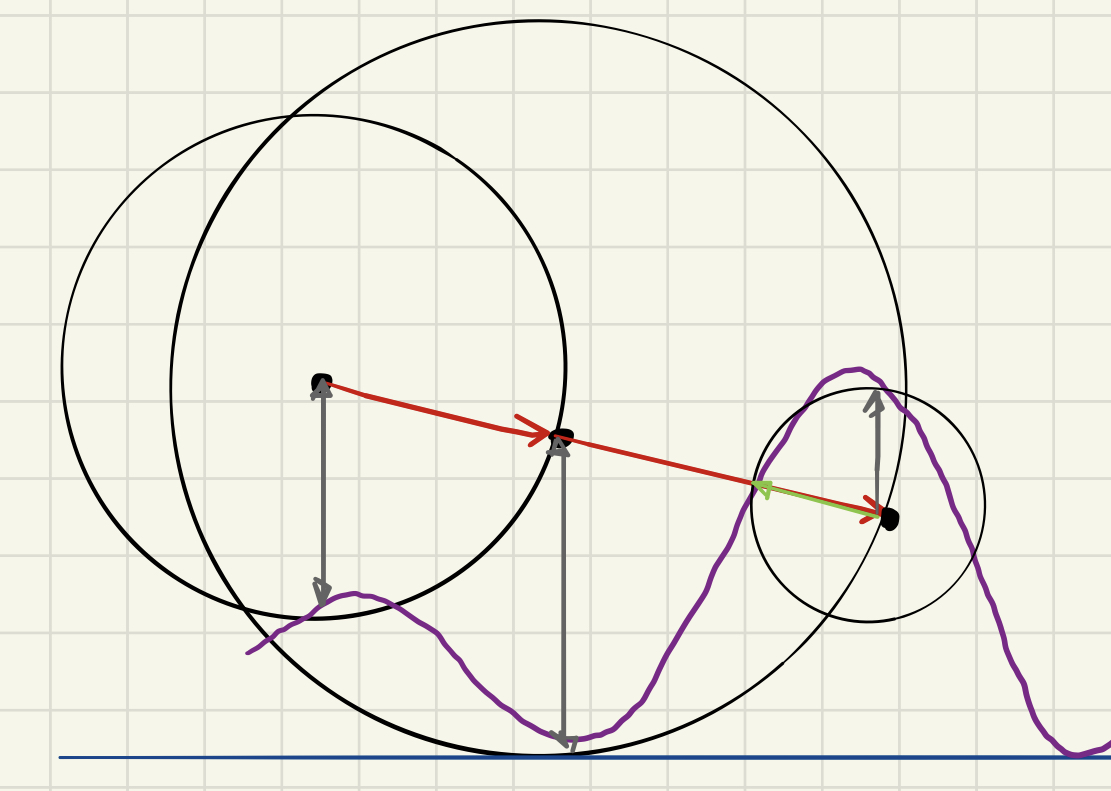
\includegraphics[width=0.4\textwidth]{secciones/imagenes/sobreestimar-interior.jpeg}\label{fig:estima_dentro}}
  \hfill
  \captionsetup{justification=centering}%,margin=2cm
  \subfloat[Estima fuera de la superficie]{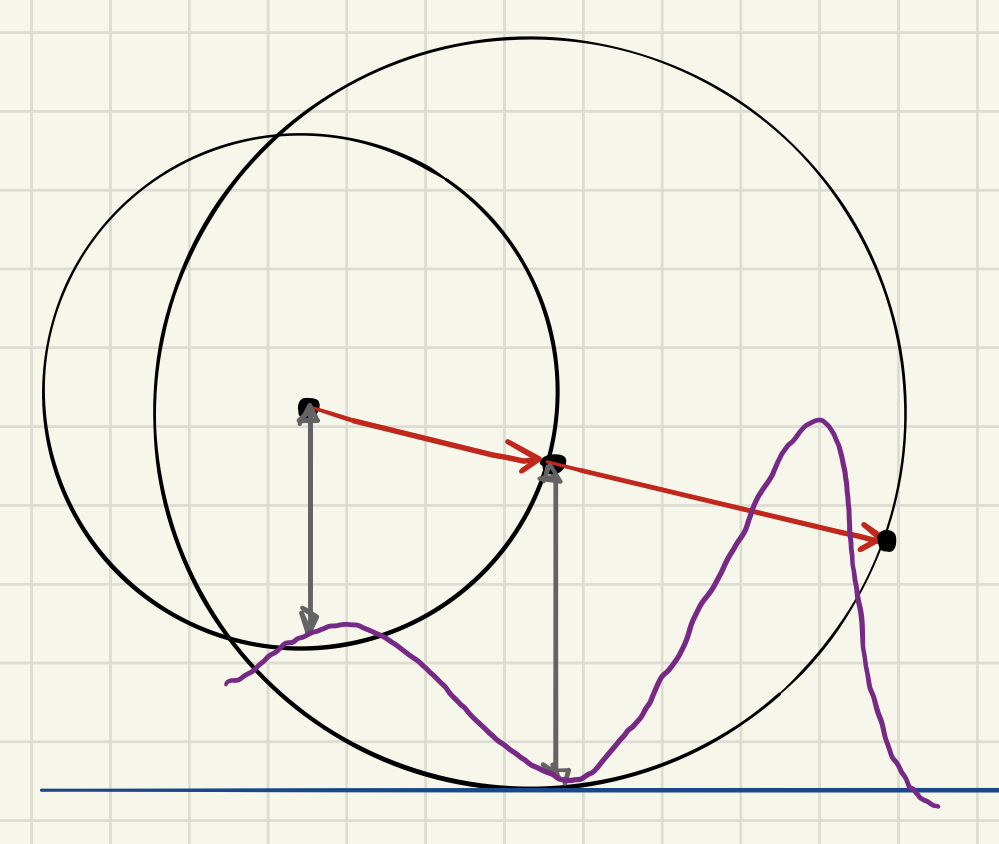
\includegraphics[width=0.4\textwidth]{secciones/imagenes/sobreestimar-exterior.jpeg}\label{fig:estima_fuera}}
  \caption{Dos formas de sobreestimar una superficie}
\end{figure}

Es difícil visualizar las circunsferencias deformadas, por lo que se ha realizado un esquema de las dos situaciones que podemos encontrar. 

\subsection{Sobrestimación en el interior}
Al poder subestimar, podemos encontrarnos en el interior, haciendo que la siguiente distancia trazada \(d_{n+1}\) sea negativa. Como teníamos definido estar sobre una superficie cuando \(d_{n+1}<\epsilon\), ya que \(d_{n+1}\) siempre es positiva cuando trazábamos desde fuera de la superficie  hacia una \textit{función de distancia con signo exacta}. Ahora que se puede sobreestimar, implicará que \(d_{n+1}\) pueda ser negativo y que debido a la condición de parada expuesta, estos puntos del interior son considerados superficie. Para solucionarlo, diremos que estamos sobre una superficie, si y solo si \( \vert d_{n+1} \vert < \epsilon\), este cambio forzará al \textit{Marcher} a que el rayo tenga que salir del interior de la superficie. Veamos el cambio en el código del algoritmo: 
\begin{lstlisting}
float SphereMarching(
    vec3 ojo, 
    vec3 direccion
){
    float distancia = 0.0;
    for(int i = 0; i < PASOS; ++i){
        vec3 p = ojo + direccion * distancia;
        float radio = escena_sdf(p);
        // Ahora esta d_{n+1} puede ser negativa, por lo que miramos el valor absoluto. 
        if(abs(radio) < EPSILON){
            return distancia;
        }
        // radio puede ser positivo o negativo, en caso de ser negativo, intentará escapar del interior hacia el exterior.
        distancia += radio;
        if(distancia >= MAXIMO) break;
    }
    return MAXIMO;
}
\end{lstlisting}
Veamos el efecto que implica este cambio sobre la deformación vista en \fullref{fig:deform}.

\begin{figure}[H]
  \centering
  \captionsetup{justification=centering}%,margin=2cm
  \subfloat[\textit{Marcher} orginal]{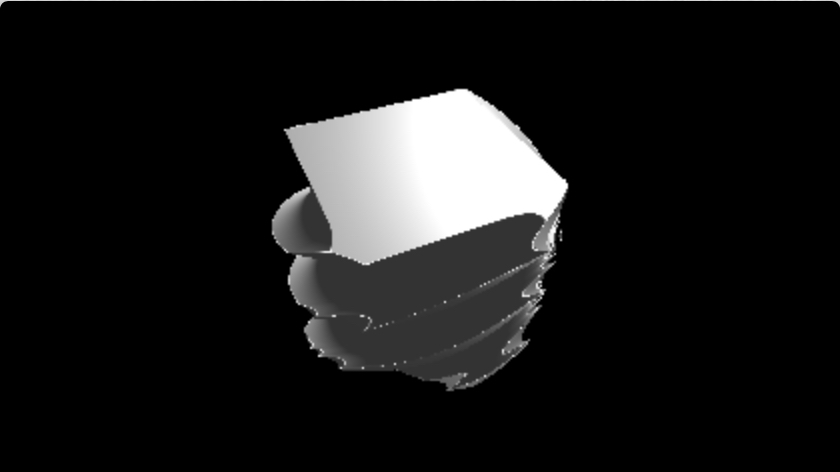
\includegraphics[width=0.4\textwidth]{secciones/imagenes/sdf_twist.jpeg}\label{fig:twistoriginal}}
  \hfill
  \subfloat[\textit{Marcher} sin sobreestimación en el interior]{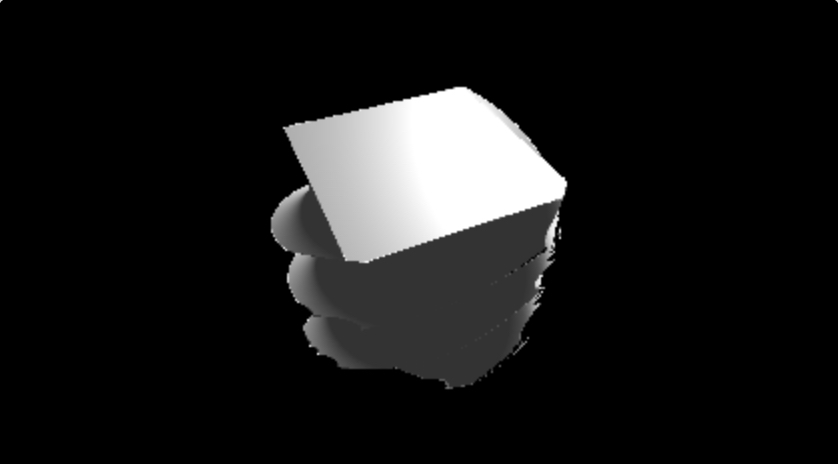
\includegraphics[width=0.4\textwidth]{secciones/imagenes/sin_sobreestimacion_interior.jpeg}\label{fig:stimateext}}
  \caption{Comparativa de los cambios realizados en el \textit{Marcher}. A la izquierda, el \textit{Marcher} original, a la derecha, el marcher con \(\vert d_{n+1}\vert < \epsilon\)}
\end{figure}

Aunque los últimos cambios son poco apreciables, podemos observar que se han reducido el número de artefactos. Por ejemplo, ahora la tapa es algo más exacta. 

\section{Sobreestimación de la distancia en el exterior}
Este segundo caso ocurre cuando la deformación aplicada hace que el rayo atraviese la superficie, como ocurre en el ejemplo \textit{\(B\)}.
Esta sobreestimación afecta considerablemente a la eficiencia del \textit{Marcher}. La solución es escalar la distancia más cercana a la superficie, obligando a que la bola deformada no pueda contener ningún punto, lo que provocará un escalado del módulo del rayo. Esto a su vez conlleva a requerir un mayor número de iteraciones.
\[d'_{n+1}=\left(\sum^{n-1}_{i=0} d_{i}\right) + f(\Vec{rayo})\cdot k \leq d_{n+1}\]
El vector \(\Vec{rayo}\) hace referencia al vector lanzado desde el ojo hasta el pixel, \(f\) es nuestra escena y \(k\in[0,1]\) es un factor de escalado para la evitar la sobreestimación, el valor es tomado de manera manual.

\begin{lstlisting}
#define FACTOR_SOBREESTIMACION k
float SphereMarching(
    vec3 ojo, 
    vec3 direccion
){
    float distancia = 0.0;
    for(int i = 0; i < PASOS; ++i){
        vec3 p = ojo + direccion * distancia;
        // Escalado del la bola
        float radio = escena_sdf(p) * FACTOR_SOBREESTIMACION;
        if(abs(radio) < EPSILON){
            return distancia;
        }
        distancia += radio;
        if(distancia >= MAXIMO) break;
    }
    return MAXIMO;
}
\end{lstlisting}
Veamos como afecta el factor \(k\) al trazado de la escena por el \textit{Marcher} sin sobreestimación en el interior.

\begin{figure}[H]
  \centering
  \captionsetup{justification=centering}%,margin=2cm
  \subfloat[k=1.0]{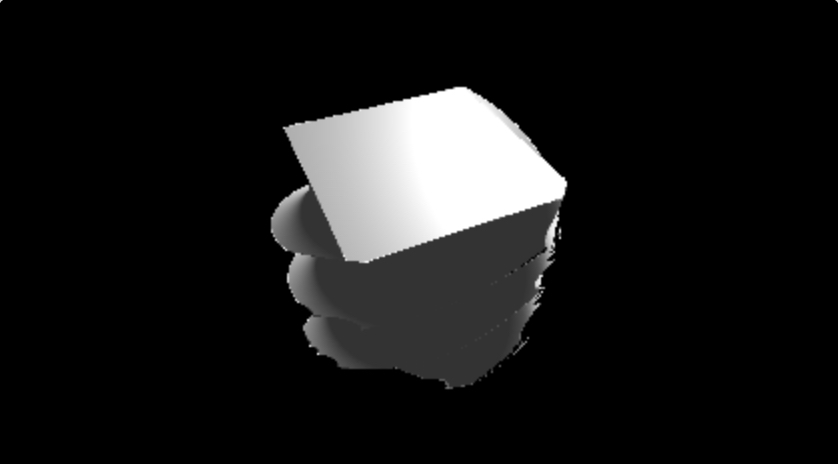
\includegraphics[width=0.3\textwidth]{secciones/imagenes/sin_sobreestimacion_interior.jpeg}\label{fig:twistoriginal1}}
  \hfill
  \subfloat[k=0.75]{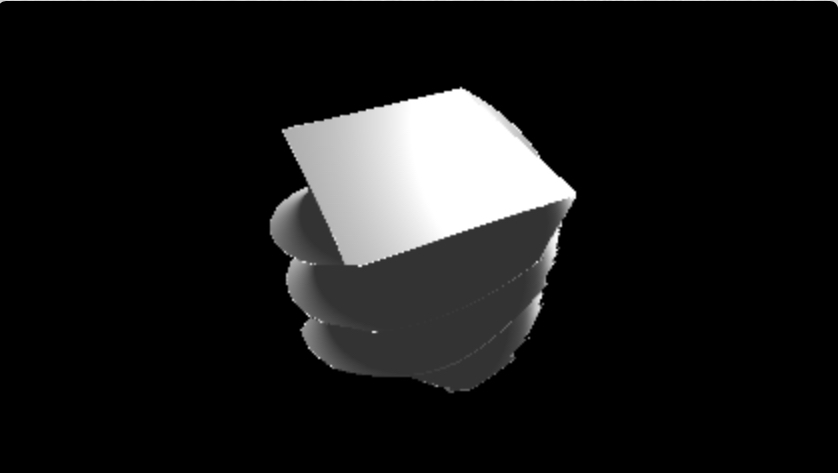
\includegraphics[width=0.3\textwidth]{secciones/imagenes/sobreestimacion_75.jpeg}\label{fig:twist75}}
  \hfill
  \subfloat[k=0.50]{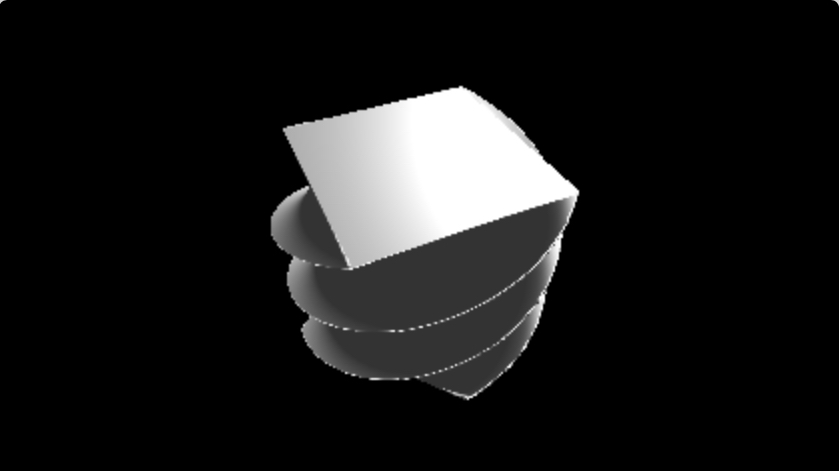
\includegraphics[width=0.3\textwidth]{secciones/imagenes/sobreestimacion_50.jpeg}\label{fig:twist50}}
  \caption{\(k\in\{1, 0.75, 0.5\}\) respectivamente sobre el \textit{Marcher} anterior}
\end{figure}

Vemos que la figura es \enquote{exacta} con \(k=0.5\) si observamos la esquina inferior izquierda de la tapadera. Este factor, o reducción de la esfera a la mitad, va a provocar que se requiera el doble de iteraciones para trazar una escena.

\subsection{Subestimación de la distancia}

Esto ocurre cuando el \textit{Marcher} ha acabado y la distancia recorrida por el rayo es inferior al plano trasero, es decir, sigue en la escena. Esto puede ocurrir principalmente cuando el rayo pasa perpendicularmente muy cerca a una superficie \(f(\Vec{rayo}) \ge \epsilon\). La siguiente imagen ilustra este problema:

\begin{figure}[H]
  \centering
  \captionsetup{justification=centering}%,margin=2cm
  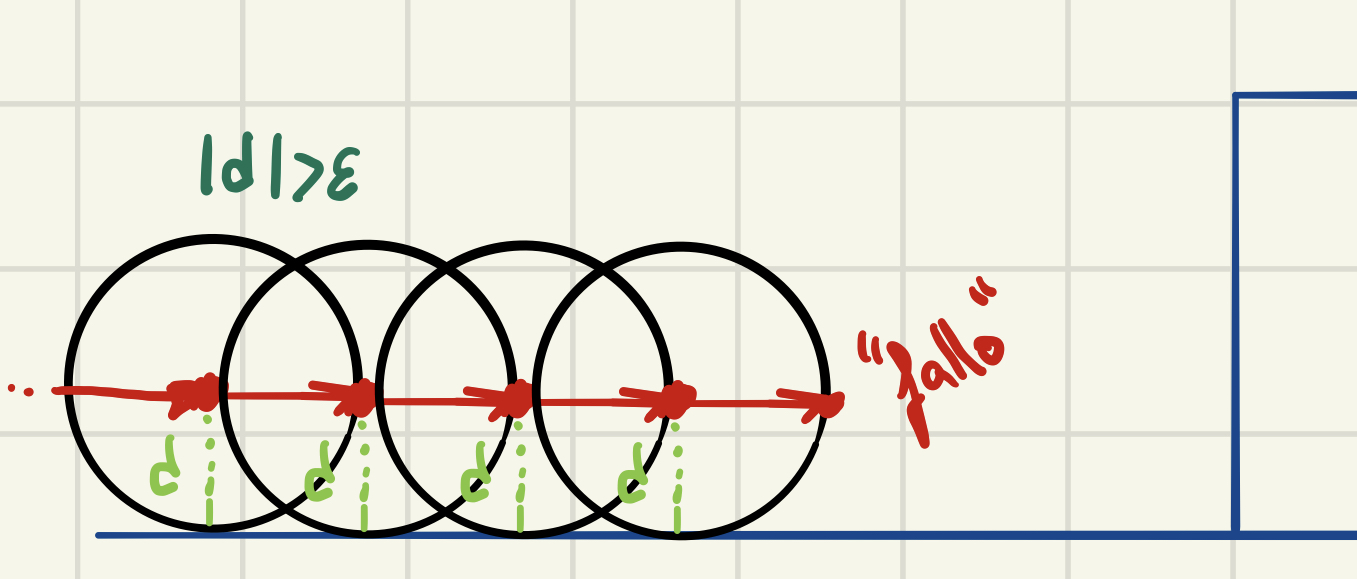
\includegraphics[width=0.8\textwidth]{secciones/imagenes/subestimacion.jpeg}\label{fig:subestimacion}
  \caption{Ejemplo de subestimación de una superficie}
\end{figure}

Estos puntos serán tratados como \textit{fallos} y por tanto, como píxeles de fondo, aunque la escena no lo fuera. Utilizar un factor de sobreestimación \(k > 1\) no sería la solución ya que crearía \textit{artefactos}, la solución propuesta es el incremento del número de iteraciones del algoritmo, en código, incrementar la definición de \textit{PASOS}, provocando un mayor gasto computacional.